% !TeX spellcheck = cs_CZ
{\tikzset{external/prefix={tikz/FYZII/}}
 \tikzset{external/figure name/.add={ch37_}{}}
%---------------------------------------------------------------------------------------------------
% file fey2ch37.tex
%---------------------------------------------------------------------------------------------------
%=========================== Kapitola Magnetické látky =============================================
\chapter{Magnetické látky}\label{fyz:IIchapXXXVII}
\minitoc
  \section{Podstata feromagnetizmu}\label{fyz:IIchapXXXVIIsecI}
  \section{Termodynamické vlastnosti}\label{fyz:IIchapXXXVIIsecII}
  \section{Hysterezní smyčka}\label{fyz:IIchapXXXVIIsecIII}
  \section{Feromagnetické látky}\label{fyz:IIchapXXXVIIsecIV}
  \section{Zvláštní magnetické látky}\label{fyz:IIchapXXXVIIsecV}

    \begin{figure}[ht!] %\ref{fyz_fig817}
      \centering
      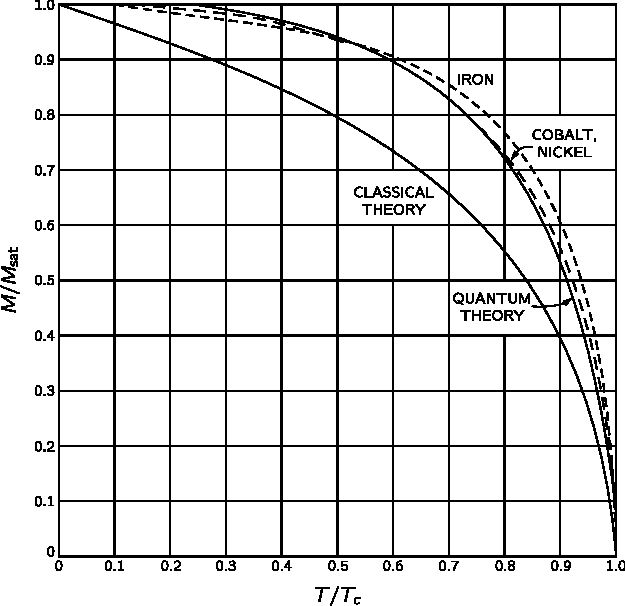
\includegraphics[width=0.7\linewidth]{fyz_fig817.pdf}
      \caption{
               (\cite[s.~707]{Feynman02})}
      \label{fyz_fig817}
    \end{figure}

    \begin{figure}[ht!]
      \centering
      \begin{tabular}{c}
        \subfloat[ ]{\label{fyz_fig818a}
          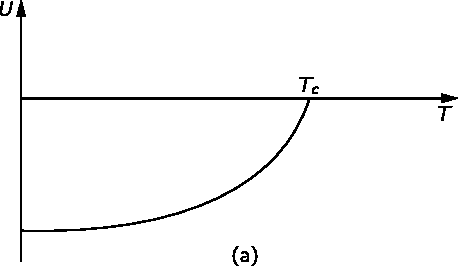
\includegraphics[width=0.7\linewidth]{fyz_fig818a.pdf}}               \\
        \subfloat[ ]{\label{fyz_fig818b}
          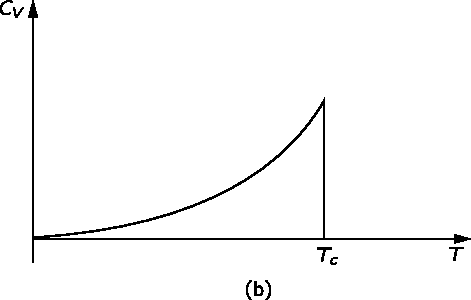
\includegraphics[width=0.7\linewidth]{fyz_fig818b.pdf}}               \\
        \subfloat[ ]{\label{fyz_fig818c}
          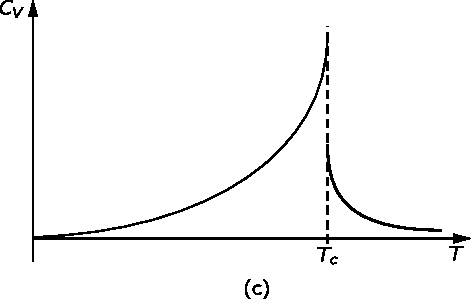
\includegraphics[width=0.7\linewidth]{fyz_fig818c.pdf}}
      \end{tabular}
      \caption{
               (\cite[s.~748]{Feynman02})}
      \label{fyz_fig818}
    \end{figure}

    \begin{figure}[ht!] %\ref{fyz_fig819}
      \centering
      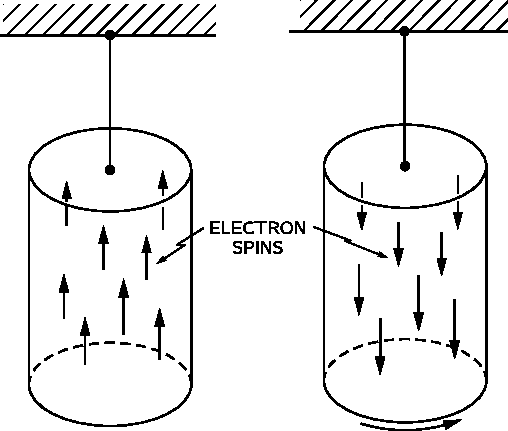
\includegraphics[width=0.7\linewidth]{fyz_fig819.pdf}
      \caption{
               (\cite[s.~707]{Feynman02})}
      \label{fyz_fig819}
    \end{figure}

    \begin{figure}[ht!] %\ref{fyz_fig820}
      \centering
      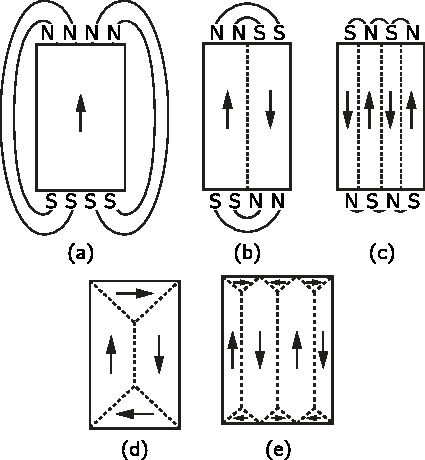
\includegraphics[width=0.7\linewidth]{fyz_fig820.pdf}
      \caption{
               (\cite[s.~707]{Feynman02})}
      \label{fyz_fig820}
    \end{figure}

    \begin{figure}[ht!] %\ref{fyz_fig821}
      \centering
      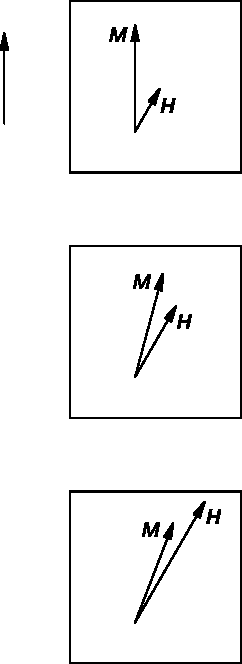
\includegraphics[width=0.7\linewidth]{fyz_fig821.pdf}
      \caption{
               (\cite[s.~707]{Feynman02})}
      \label{fyz_fig821}
    \end{figure}

    \begin{figure}[ht!] %\ref{fyz_fig822}
      \centering
      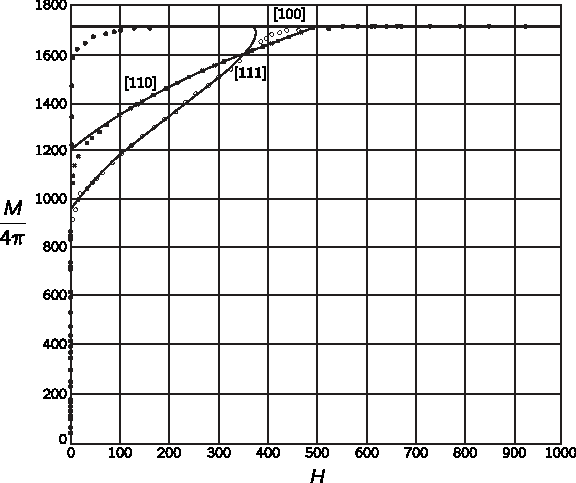
\includegraphics[width=0.7\linewidth]{fyz_fig822.pdf}
      \caption{
               (\cite[s.~707]{Feynman02})}
      \label{fyz_fig822}
    \end{figure}

    \begin{figure}[ht!]
      \centering
      \begin{tabular}{c}
        \subfloat[ ]{\label{fyz_fig823a}
          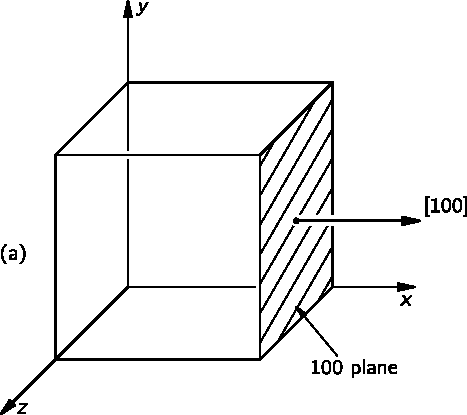
\includegraphics[width=0.7\linewidth]{fyz_fig823a.pdf}}               \\
        \subfloat[ ]{\label{fyz_fig823b}
          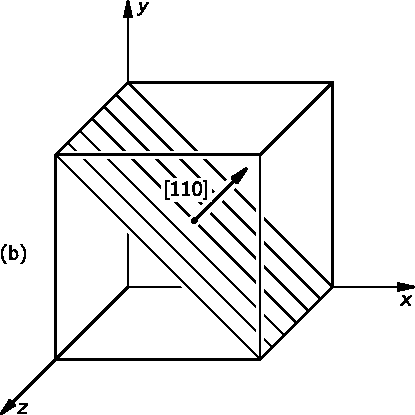
\includegraphics[width=0.7\linewidth]{fyz_fig823b.pdf}}               \\
        \subfloat[ ]{\label{fyz_fig823c}
          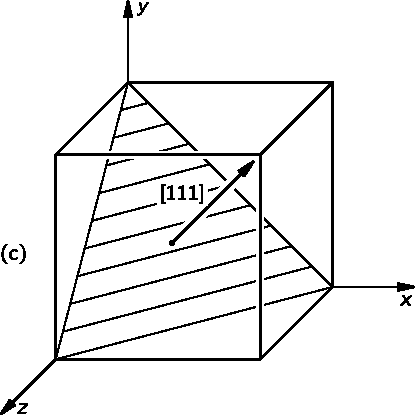
\includegraphics[width=0.7\linewidth]{fyz_fig823c.pdf}}
      \end{tabular}
      \caption{
               (\cite[s.~748]{Feynman02})}
      \label{fyz_fig823}
    \end{figure}

    \begin{figure}[ht!]
      \centering
      \begin{tabular}{c}
        \subfloat[ ]{\label{fyz_fig824a}
          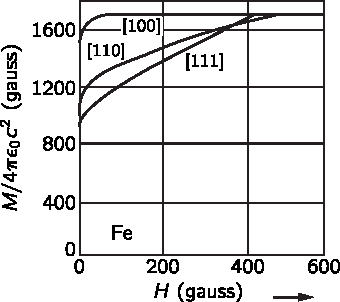
\includegraphics[width=0.7\linewidth]{fyz_fig824a.pdf}}               \\
        \subfloat[ ]{\label{fyz_fig824b}
          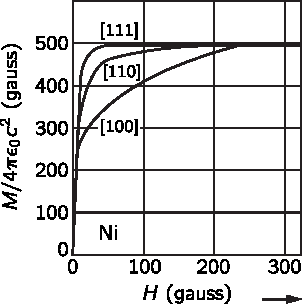
\includegraphics[width=0.7\linewidth]{fyz_fig824b.pdf}}               \\
        \subfloat[ ]{\label{fyz_fig824c}
          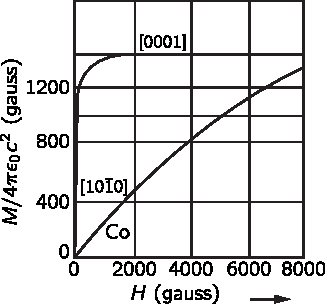
\includegraphics[width=0.7\linewidth]{fyz_fig824c.pdf}}
      \end{tabular}
      \caption{
               (\cite[s.~748]{Feynman02})}
      \label{fyz_fig824}
    \end{figure}

    \begin{figure}[ht!] %\ref{fyz_fig825}
      \centering
      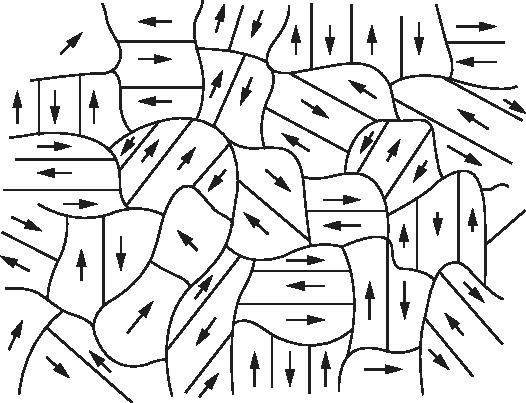
\includegraphics[width=0.7\linewidth]{fyz_fig825.pdf}
      \caption{
               (\cite[s.~707]{Feynman02})}
      \label{fyz_fig825}
    \end{figure}

    \begin{figure}[ht!] %\ref{fyz_fig826}
      \centering
      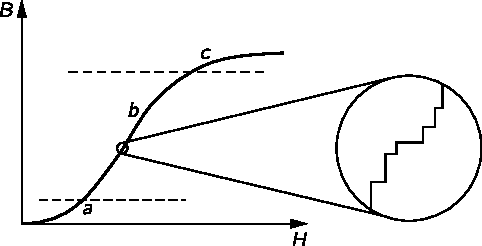
\includegraphics[width=0.7\linewidth]{fyz_fig826.pdf}
      \caption{
               (\cite[s.~707]{Feynman02})}
      \label{fyz_fig826}
    \end{figure}

    \begin{figure}[ht!] %\ref{fyz_fig827}
      \centering
      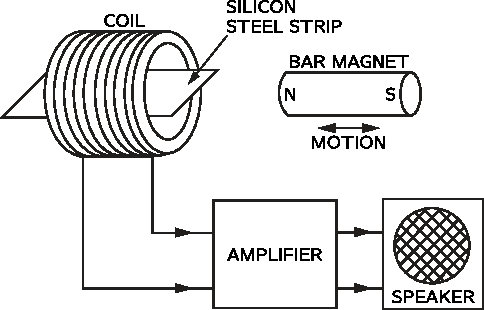
\includegraphics[width=0.7\linewidth]{fyz_fig827.pdf}
      \caption{
               (\cite[s.~707]{Feynman02})}
      \label{fyz_fig827}
    \end{figure}

    \begin{figure}[ht!] %\ref{fyz_fig828}
      \centering
      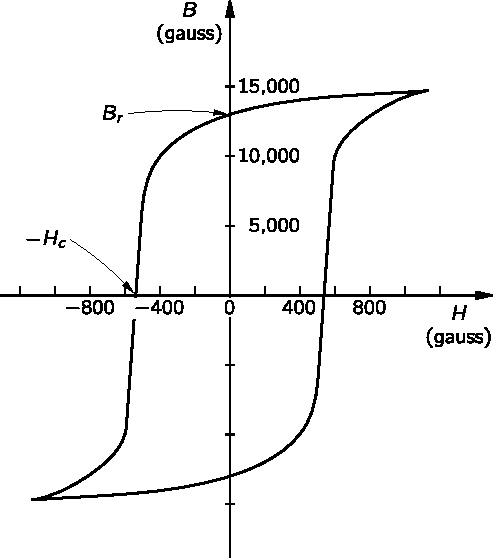
\includegraphics[width=0.7\linewidth]{fyz_fig828.pdf}
      \caption{
               (\cite[s.~707]{Feynman02})}
      \label{fyz_fig828}
    \end{figure}

    \begin{figure}[ht!] %\ref{fyz_fig829}
      \centering
      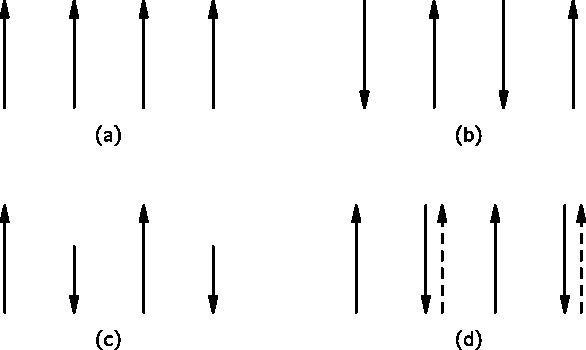
\includegraphics[width=0.7\linewidth]{fyz_fig829.pdf}
      \caption{
               (\cite[s.~707]{Feynman02})}
      \label{fyz_fig829}
    \end{figure}
s
    \begin{figure}[ht!] %\ref{fyz_fig830}
      \centering
      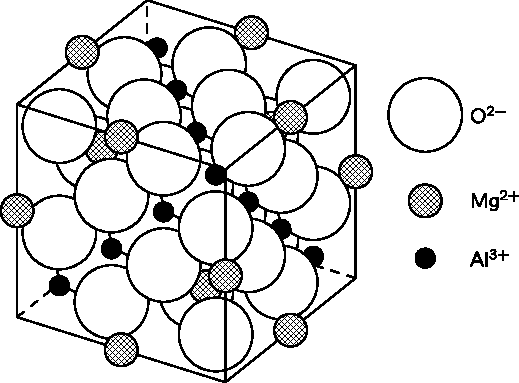
\includegraphics[width=0.7\linewidth]{fyz_fig830.pdf}
      \caption{
               (\cite[s.~707]{Feynman02})}
      \label{fyz_fig830}
    \end{figure}

} %tikzset
%---------------------------------------------------------------------------------------------------
\printbibliography[title={Seznam literatury},heading=subbibliography]
\addcontentsline{toc}{section}{Seznam literatury}